%----------------------------------------------------------------------------
\chapter{Test Framework}
%----------------------------------------------------------------------------

This chapter presents the design and implementation of the test framework that facilitates the automatic deployment of the sample application and running the measurements to determine the dependability metrics of the system.

%----------------------------------------------------------------------------
\section{Design}
%----------------------------------------------------------------------------

Consistency is essential when testing. In order to get meaningful results that can be later used to evaluate the implementation and to draw conclusions, a well defined framework is needed that sets clear boundaries on how the results are acquired. The quality of the testing and measurement greatly depends on the way these activities are executed, which means that a detailed design of the framework is vital.

%\begin{itemize}
%	\item why is a framework needed
%	\item test framework architecture
%	\item what is the test objective?
%	\item what to test? - dependability metrics! - which ones?, how?
%	\item need to monitor the application metrics, state --> need for monitoring system
%	
%	\item how does running tests affect the result
%\end{itemize}

%----------------------------------------------------------------------------
\subsection{Test objective}
%----------------------------------------------------------------------------

The first thing to specify when designing a test framework is the test objective. This highly affects the way the framework should be planned and created.

The goal of the framework is to measure the dependability metrics of the sample application to reveal weak spots and to discover opportunities to improve the dependability of the application.

%----------------------------------------------------------------------------
\subsection{Requirements}
%----------------------------------------------------------------------------

The design of the test framework was driven by several requirements to create an architecture that facilitates achieving the test objective defined in the previous section.

\paragraph{Configurable} In order to support various kinds of test scenarios, the framework should be highly configurable. This characteristic also makes the testing system more reusable and generic, so it is not closely tailored to the sample application described in this project.

\paragraph{Reproducible} The framework should function in a fairly deterministic way. This means that any two test executions with the same configuration should produce approximately the same results. As the applications that the framework is designed to evaluate are Kubernetes based, distributed systems, requiring complete deterministic behavior of the framework is not realistic. There are several things that can introduce a slight level of randomness to the application. For example the state of the network between the components or the way the fault injection logic inserts anomalies into the system (further details in section \ref{test-design-fault-injector}).

\paragraph{Automated} The usability of the framework greatly depends on how much manual interaction is needed for it produce results. Ideally, the framework should not require any human actions to be able to function after the configurations are correctly set. Automation enables the users of the framework to define multiple test scenarios with different configurations, collect them into a script and start all the measurements with only one command. Furthermore, if the framework is able to operate autonomously once it gets the right inputs, it can be integrated into existing pipelines (Continuous Integration, Continuous Delivery) to act as a quality gateway before an application is deployed into production.

%\begin{itemize}
%	\item Reproducible
%	\item Automated
%	\item Configurable
%\end{itemize}

%----------------------------------------------------------------------------
\subsection{Framework workflow}
%----------------------------------------------------------------------------

%	\item Introduce abstract workflow \begin{enumerate}
%		\item Prepare infrastructure and application
%		\item Generate load
%		\item Inject faults
%		\item Collect metrics -  need to monitor the application metrics, state --> need for monitoring system
%		\item Store results
%	\end{enumerate}


Considering the test objective and the requirements described in the previous sections, the functional workflow of the testing framework can be seen in Figure \ref{fig:test_framework_workflow}.

\begin{figure}[h]
	\centering
	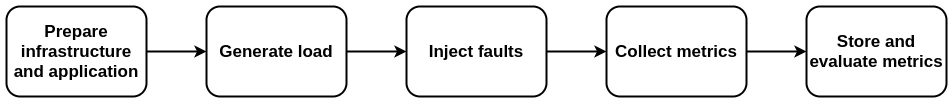
\includegraphics[width=140mm, keepaspectratio]{figures/test_framework_workflow.png}
	\caption{Test framework workflow}
	\label{fig:test_framework_workflow}
\end{figure}

As per this design, the framework should first prepare the environment for testing. This consists of setting up the Kubernetes infrastructure that the application will run on and starting the deployed application in this environment. After the application is running, in order to trigger to trigger task executions, a subsystem generates and sends load to the application. To better understand how the system under test behaves, different kinds of faults and anomalies are introduced to the system while the executions and possibly the load generation are in progress. The framework constantly collects the exposed metrics from the application and the infrastructure to gain insights about how the system manages to handle the implanted anomalies. After the load generation and the task executions are done, the metrics get stored and evaluated.

%----------------------------------------------------------------------------
\subsection{Architecture}
%----------------------------------------------------------------------------

The architecture of the test framework that facilitates the previously defined workflow is displayed in Figure \ref{fig:test_framework_arch}.

\begin{figure}[h]
	\centering
	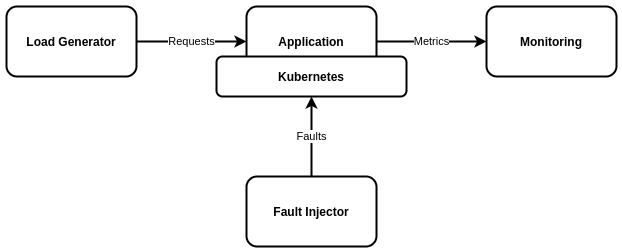
\includegraphics[width=140mm, keepaspectratio]{figures/test_framework_arch.png}
	\caption{Test framework architecture}
	\label{fig:test_framework_arch}
\end{figure}

The framework consists of three main components: the load generator, the fault injector and the monitoring subsystem. Each is described in the following sections.


%\begin{itemize}
%	\item architecture DIAGRAM
%	\item describe what each component does
%\end{itemize}


%----------------------------------------------------------------------------
\subsection{Load Generator}
%----------------------------------------------------------------------------

%\begin{itemize}
%	\item send HTTP requests to the backend according to pattern (uniform distribution)
%\end{itemize}

The responsibility of the load generator component is to simulate real world workload on the sample application. This way the framework can better assess the actual dependability characteristics of the system.

As the sample application (more precisely the backend) accepts user inputs in the form of HTTP requests, the load generator component should be able to produce correctly built up HTTP requests and send them to the application. This will trigger task executions and multiple worker instance deployments in case the requests are sent more frequently than a single worker could execute them one by one without leaving any tasks waiting in the message queue.

%----------------------------------------------------------------------------
\subsection{Parameters}
%----------------------------------------------------------------------------

% input value
% wait time between requests - different distributions
% number of simulated users

There are several ways to customize the way that load generation happens and how much workload it causes to the system under test.

\paragraph{Task input value} Probably the most trivial way is to change the task input value in the requests. As described in section \ref{impl-backend-interfaces}, the \texttt{input} field in the request JSON determines which Fibonacci number is calculated by a worker component. This means the time a worker instance spends on executing a task can be manipulated by the input value.

\paragraph{Request frequency} Another method that the load generator can exploit to control the workload on the system is to wait different amounts of time between sending individual requests. This can also model how real users would use the application. The wait time between requests can be a constant value, but in fact, it can be calculated based upon any arbitrary logic. Generally, various kinds of distribution functions are used to determine the request frequency.

\paragraph{Parallelism} To increase the workload on the system, multiple requests can be sent by the load generator in parallel. Using this together with increasing the request frequency can greatly intensify the load on the application. Similarly to the request frequency, the amount of requests to send in parallel can be calculated using any logic.


%----------------------------------------------------------------------------
\subsection{Fault Injector} \label{test-design-fault-injector}
%----------------------------------------------------------------------------

\begin{itemize}
	\item inject faults on different levels (Pod, Network, CPU, Memory)
	\item periodic fault injection
\end{itemize}


%----------------------------------------------------------------------------
\subsubsection{Fault Profiles}
%----------------------------------------------------------------------------

\begin{itemize}
	\item list fault profiles and justification
\end{itemize}


%----------------------------------------------------------------------------
\subsection{Monitoring}
%----------------------------------------------------------------------------



%----------------------------------------------------------------------------
\section{Implementation}
%----------------------------------------------------------------------------

\begin{itemize}
	\item Test environment locally or in cloud
	\item AWS infrastructure
	\item CF template
\end{itemize}

%----------------------------------------------------------------------------
\subsection{Load generation}
%----------------------------------------------------------------------------

\begin{itemize}
	\item locust
	\item usermodel
	\item parameterization
\end{itemize}

%----------------------------------------------------------------------------
\subsection{Fault Injection}
%----------------------------------------------------------------------------

\begin{itemize}
	\item deploy Chaos Mesh
	\item define chaos experiments according to fault profiles (show one as example)
	\item describe the usage of helm to deploy faults
\end{itemize}

%----------------------------------------------------------------------------
\subsection{Measurement} \label{measurement-impl}
%----------------------------------------------------------------------------

\begin{itemize}
	\item Deploy tools \begin{itemize}
		\item Prometheus
		\item Prometheus Adapter
		\item Promethues Blackbox Exporter
		\item Grafana
	\end{itemize}
	\item prometheus annotations, scrape config
	\item measurement sequence - what is the purpose of this
\end{itemize}

%----------------------------------------------------------------------------
\subsubsection{Metrics}
%----------------------------------------------------------------------------

\begin{itemize}
	
	\item dependability metrics in PromQL
	\item justify the 15 multiplier - it is the prometheus scrape interval
\end{itemize}







%----------------------------------------------------------------------------
\subsection{Kubedepend}
%----------------------------------------------------------------------------

\begin{itemize}
	\item what it is used for?
	\item facilitates automatic load generation, fault injection, collecting results
	\item describe its workflow
	\item purpose of waiting for stable system state
	\item prometheus metrics
	\item parameters (click)
\end{itemize}

%----------------------------------------------------------------------------
\subsection{CI/CD Pipeline} \label{cicd}
%----------------------------------------------------------------------------

\begin{itemize}
	\item Steps and what do they do
	\item image about jenkins pipeline steps
	\item parameters - passed to kubedepend
\end{itemize}